\section{Photometer}

\subsection{Introduction}

\begin{figure}[H]
    \centering
    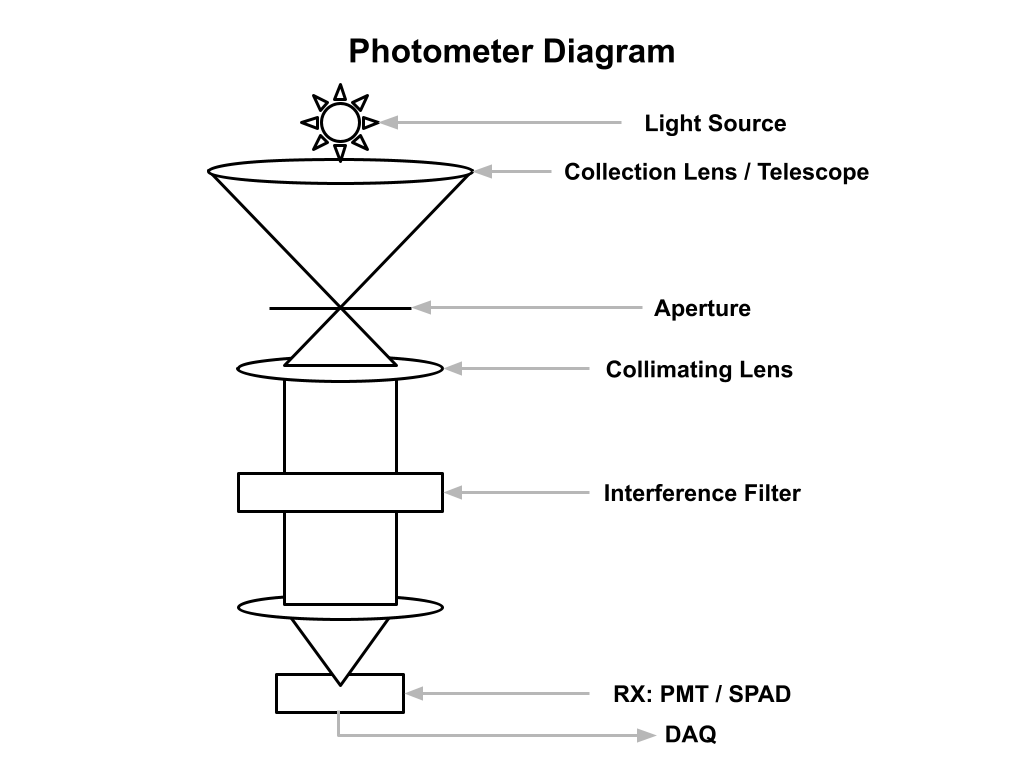
\includegraphics[width=0.75\linewidth]{images/photometer_diagram.png}
    \caption{A diagram of a photometer.}
    \label{fig:photometer_diagram}
\end{figure}

A photometer measures the number of photons from a source. The receiver can either be a \textbf{photomultiplier tube (PMT)} or a \textbf{single-photon avalanche diode (SPAD)}. A PMT is a single-element instrument that counts individual photons precisely.

\vsp

A \textbf{charge-coupled device (CCD)} is an array of sensors that take a 2D image of incoming photons, making it a multi-channel device. Scientific-grade CCDs are more expensive than PMTs.

\begin{table}[H]
    \centering
    \begin{tabular}{c|c|c}
        Feature             & CCD                            & PMT             \\
        \hline
        \hline
        Detection type      & Multi-channel                  & Single-channel  \\
        Sensitivity (QE)    & Very high (\textgreater{90\%}) & Lower (20-40\%) \\
        Internal gain       & Low/none                       & Extremely high  \\
        Temporal resolution & Slow                           & Extremely fast
    \end{tabular}
\end{table}

\textbf{Quantum efficiency (QE)} measures how sensitively the detector is to photons. Thus, a QE of 90\% means that the detector converts 90\% of incoming photons into electrons.

\vsp

The \textbf{internal gain} of a detector is the amplification of the singal. Because the PMT works in a very high temporal resolution (collecting data rapidly), it needs to amplify the signal considerably.

\vsp

A CCD collects photons over a much larger range of time, called the \textbf{integration time}. Thus, a CCD can image very dim astronomical objects by letting photons accumulate over this long integration time.

\vsp

Some abbreviations:
\begin{itemize}
    \item IF = Interference Filter
    \item RX = Receiver
    \item TX = Transmitter
\end{itemize}

\subsection{Forward Model}

A \textbf{forward model} is a mathematical or quantitative description of the problem you're solving. One can use synthetic data and example numbers to test. We will explore the forward model of a photometer in the following sections.

\subsubsection{Photon Count}

\begin{equation*}
    N = N_{\text{signal}} + N_{\text{noise}}
\end{equation*}

where

\begin{itemize}
    \item $N$ is the total number of photons,
    \item $N_{\text{signal}}$ is the number of photons from the desired source,
    \item $N_{\text{noise}}$ is the number of photons from other (undesirable) sources.
\end{itemize}

\subsubsection{Noise Count}

\begin{equation*}
    N_{\text{noise}} = N_C \Delta t
\end{equation*}

where

\begin{itemize}
    \item $N_C \, [\text{counts/s}]$ is the noise count rate,
    \item $\Delta t \, [s]$ is the \textbf{integration time} (the time interval at which the detector collects photons).
\end{itemize}

\subsubsection{Signal Count}

\begin{align*}
    N_{\text{signal}} & = BA\Delta t \, \Omega T_A \nu_{RX}  \\
    \Omega            & = \frac{A}{r^2} = 2\pi(1-\cos\alpha)
\end{align*}

where

\begin{itemize}
    \item $B \, [\text{photons}/(\text{s} \cdot \text{m}^2 \cdot \text{str})]$ is a constant,
    \item $A \, [\text{m}^2]$ for $N_{\text{signal}}$ is the area of the telescope,
    \item $\Delta t \, [s]$ is the integration time,
    \item $\Omega \, [\text{str}]$ is the solid angle,
    \item $T_A$ is the atmospheric transmission,
    \item $\nu_{RX}$ is the receiver efficiency,
    \item $A$ for $N_{\text{noise}}$ is the area of the detector,
    \item $r$ is the focal length of the telescope,
    \item $\alpha$ is the half-angle of the cone of light collected by the telescope, also known as the field of view.
\end{itemize}

Note: $A\Omega$ is a conserved quantity called the \textbf{etendue}.